\documentclass[a4paper, 12pt]{article}
\usepackage[utf8]{inputenc}
\usepackage[T1]{fontenc}
\usepackage[french]{babel}
\usepackage{graphicx}
\usepackage{amsmath}
\usepackage{hyperref}
\usepackage{lmodern}
\usepackage{moreverb}
\usepackage{multicol}


\usepackage[a4paper,left=2cm,right=2cm,top=2cm,bottom=2cm]{geometry}

\pagestyle{headings}
\pagestyle{plain}


\setcounter{secnumdepth}{4}
\setcounter{tocdepth}{4}
\makeatletter


\makeatother

\makeatletter
\def\toclevel@subsubsubsection{4}
\def\toclevel@paragraph{5}
\def\toclevel@subparagraph{6}
\makeatother

\setlength{\parindent}{0cm}
\setlength{\parskip}{1ex plus 0.5ex minus 0.2ex}
\newcommand{\hsp}{\hspace{20pt}}
\newcommand{\HRule}{\rule{\linewidth}{0.5mm}}

\begin{document}

\begin{titlepage}
  \begin{sffamily}
  \begin{center}

   
    \textsc{\LARGE }\\[2cm]

    \textsc{\Large Compte rendu de Réunion}\\[1.5cm]
    \textsc{\Medium Rédigé par Ghilas MEZIANE}

    % Title
    \HRule \\[0.4cm]
    { \huge  \textsc{StellaStone} \\
    \textsc{\Large By Novus}\\ [0.4cm] }
	
    \HRule \\[2cm]
    \textsc {Idriss BENGUEZZOU\\Ghilas MEZIANE}
 \begin{figure}
     \centering
    
\includegraphics[scale=0.2]{logoUJM.png}
     \label{fig:ujm_logo}
 \end{figure}

    \vfill

    % Bottom of the page
    {\large {} 20/01/2023}

  \end{center}
  \end{sffamily}
\end{titlepage}


\newpage
\tableofcontents

\newpage

\section{Réunion du Vendredi 20/01}

Cette réunion est la première organisée par le groupe Novus depuis la fin de la première partie du projet. L'objectif de cette réunion était de lister les fonctionnalités qui devront êtres mises en place durant cette phase de développement ainsi que de choisir le moteur de jeu que l'on utilisera et donc le langage de développement.

Cette réunion à été réalisée en deux fois, nous avions pu noter certains points lors du cours de projet intégré le Lundi 16 janvier 2023. 
Cependant, il nous a fallu mener quelques recherches quant au choix du moteur de jeux, c'est pourquoi nous avons décidé de tenir une seconde réunion le 21/01/2023 afin de prendre les décisions nécessaires. 


\subsection{Choix du moteur de jeu}

Lors de la première discussion que l'on a pu avoir le Lundi 16 janvier 2022, nous avions décidé de tester différents moteurs de jeu, tel que Unity, Unreal Engine, CryEngine, Godot...

Lors de la première partie de ce projet les membres de Novus avaient dans un premier temps décidé de réaliser StellaStone à l'aide d'Unreal Engine. En effet, Unreal Engine est l'un des moteurs les plus puissants et l'un des plus utilisés sur le marché avec des fonctionnalités très avancées pour les graphismes.

Cependant, alors que le binôme se questionnait quant à la pertinence de ce choix, Idriss a souligné que Unity est plus facile à utiliser pour les développeurs débutants et qu'il jouit d'une communauté de développeurs active, d'innombrables tutoriels sont accessibles sur le net, et une large documentation est disponible.

Les performances ont également été discutées, les deux parties ont convenu que les moteurs de jeu modernes ont tendance à être assez gourmands et que la performance dépendra principalement de la puissance des machines de développement.

Les deux parties ont également discuté de la facilité de prise en main des moteurs de jeu et ont convenu que Unity est plus facile à prendre en main comparé à Unreal Engine.

Enfin, Idriss a souligné le fait qu'il fallait découvrir le langage C\# qui est le langage pris en charge par Unity. Au final, le binôme a décidé de choisir Unity pour le développement de l'application StellaStone.


\subsection{Fonctionnalités à implémenter}

À l'issue de cette réunion, nous avons donc retenu un certain nombre de fonctionnalités à partir du documents de spécifications des exigences produit lors de la première partie du projet. 

Les fonctionnalités à implémenter seront donc les suivantes : \\
\begin{itemize}
    \item \textbf{l'authentification} permettant de s'inscrire et de se connecter (exigence : EI-AUT / EI-AIN / EI-ACO), \\ 
    \item \textbf{la construction} de la fusée avec les modes Aventure et Réaliste (exigence : EI-CDF / EI-CDF-MR / EI-CDF-MA),\\
    \item \textbf{la réalisation} du voyage avec les options de pilotage et d'auto-pilotage en mode Aventure et Réaliste (exigence : EI-VOY / EI-VOY-REA / EI-VOY-AVE),\\
    \item \textbf{l'interface Accueil} étant primordial nous avons décider de retirer l'aspect collaboratif (exigence : EI-ACC-COL), nous gardons en revanche toute les autres fonctionnalité de l'Accueil (exigence : EI-ACC),\\
    \item \textbf{le profil et les paramètres} ont également été retenu, pour l'interface profil la majorité des fonctionalité on été retiré (exigence retnue :  EI-PRO-VC / EI-PRO-NAV), pour ce qui est des paramètre l'intégralité des exigences ont été retenu (exigence : EI-PRO-PA). \\
\end{itemize}

Nous avons cherché à maintenir un équilibre entre la faisabilité, la difficulté technique et le temps disponible pour réaliser le projet. C'est pourquoi nous avons sélectionné les fonctionnalités en fonction de ces critères, en essayant de conserver un maximum de fonctionnalités.

Cependant, il est possible que nous soyons amenés à retirer certaines fonctions si nous jugeons qu'il sera impossible de les implémenter dans les délais impartis.

\subsection{Estimations COCOMO II}

Dans le cadre de notre projet, nous avons utilisé un outil en ligne pour générer des estimations de coût pour la réalisation du projet. L'image ci-dessous représente les paramètres entrés dans cet outil pour notre projet. Il montre les différents facteurs pris en compte pour générer les estimations de coût, tels que la taille du projet, le degré de complexité et les caractéristiques de l'équipe de développement. Ces paramètres ont été soigneusement sélectionnés en fonction des besoins et des caractéristiques de notre projet.

 \begin{figure}[!h]
    \centering
    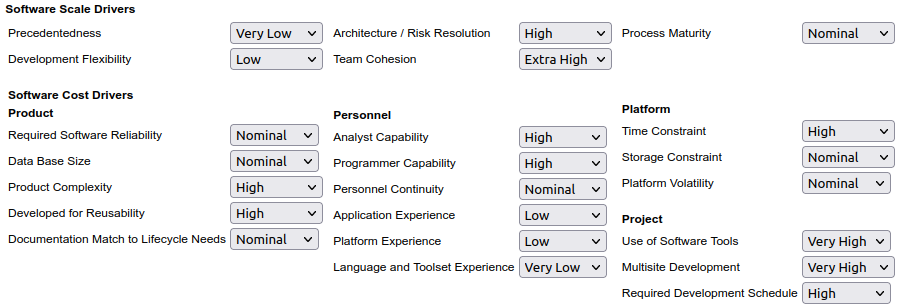
\includegraphics[scale=0.5]{ccmo.png}
    \label{fig:Le_planning}
    \caption{Paramètres de l'estimation}
\end{figure}

Par exemple, le paramètre Precedentedness est mis à Very low car nous n'avons pas eu l'occasion de développer une telle application.

Le paramètre Development Flexibility est quant à lui mis à Low car la première partie de ce projet nous a permis de fixer le cadre du projet et de nous guider tout au long de ce deuxième semestre. Néanmoins nous ne respecterons pas à 100\% les exigences spécifiées, c'est pour cela que nous n'avons pas mis ce paramètre à Very Low.

Le paramètre Architecture/Risk Resolution est mis à High, car nous avons listé différents tests pour anticiper toutes les erreurs possibles, nous avons établi plusieurs diagrammes de séquence, et nous avons également pris en compte la protection des données et leur utilisation lors du premier semestre. 

\newpage
Voici une première estimation du coût de réalisation du projet StellaStone, modélisée à l'aide de l'outil COCOMO II en ligne, qui nous fournit une estimation basée sur une prédiction de 8000 lignes de code. 


 \begin{figure}[!h]
    \centering
    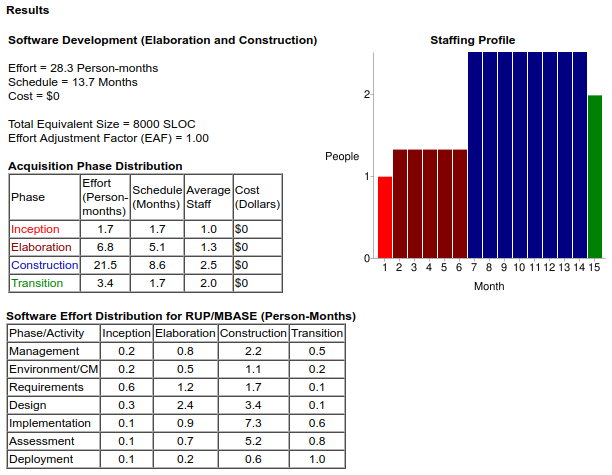
\includegraphics[scale=0.75]{ccmo3.png}
    \label{fig:Le_planning}
    \caption{8000 lignes de codes}
\end{figure}

\newpage

Une seconde estimation basée sur une prédiction stipulant que nous développerons 3000 lignes de code, nous permet de générer le rapport suivant :  
 \begin{figure}[!h]
    \centering
    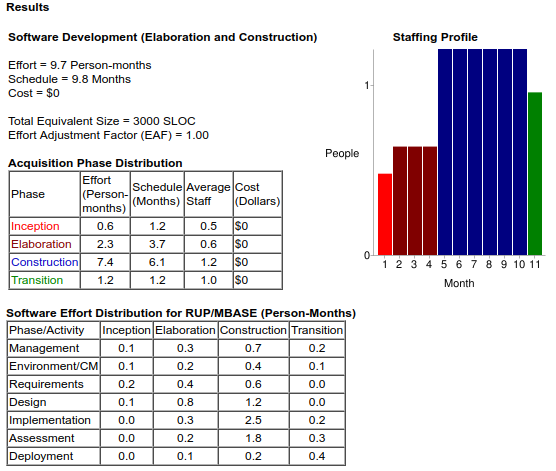
\includegraphics[scale=0.75]{ccmo2.png}
    \label{fig:Le_planning}
    \caption{3000 lignes de codes}
\end{figure}

\newpage
\section{Le planning}

Le planning mis en place reprend les principales fonctionnalités qui devront être implémenté. Bien entendu ce planning sera amené à changé durant le semestre.

Notre planning, est séparé en quatre "Sprint" (phase) :

 \begin{figure}[!h]
    \centering
    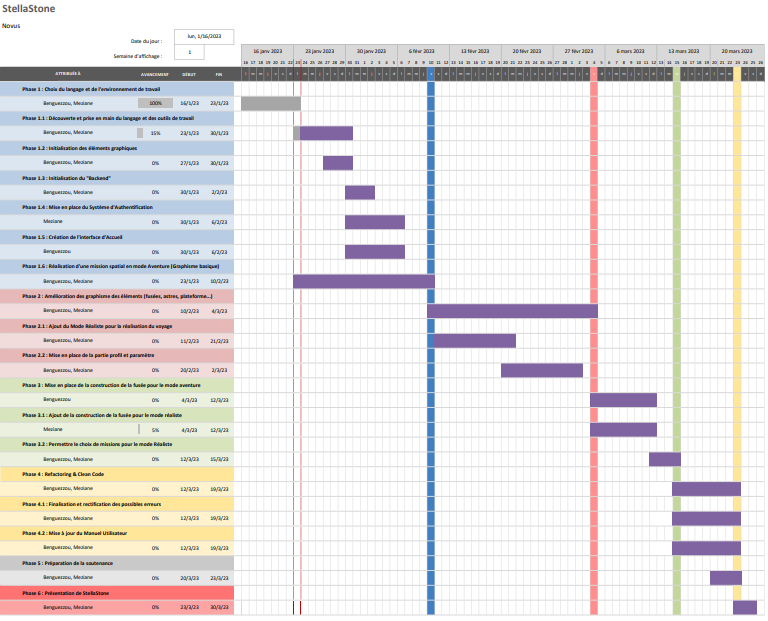
\includegraphics[scale=0.65]{Le planning.png}
    \label{fig:Le_planning}
    \caption{Un premier Diagramme de Gantt}
\end{figure}

\section{Planification du travail de la semaine à venir}

Dans la continuité du premier semestre, nous continuerons à utiliser git pour le développement de StellaStone. Les réunions auront lieu tous les vendredis en présentiel ou à distance en fonction de nos disponibilités. 

Comme nous l'avons mentionné plus haut, nous avons divisé le projet en 4 sprints. Pour la première phase, notre objectif principal sera de se familiariser avec le nouveau langage et l'environnement de travail proposé par Unity, ainsi que d'implémenter les fonctionnalités majeures du projet sans trop nous attarder sur le design du logiciel.

L'objectif de cette semaine est donc dans un premier temps de découvrir et de prendre en main les outils proposés par Unity et de se familiariser avec eux. Dans le cas où nous ne rencontrions pas de problèmes, nous pourront commencer à initialiser le projet en créant un environnement 3D et en initialisant la base de données. 

L'objet de la prochaine réunion, qui se tiendra le 27/01/2023, sera donc de mettre en commun l'avancée des deux membres du groupe et de partager les difficultés rencontrées. À l'issue de cette prochaine réunion, des règles et conventions de clean code devront être mises en place et respectées tout au long du développement de StellaStone.

\end{document}